\documentclass[a4paper, 12pt]{article}
%\documentclass{article}
\usepackage{amsmath}
\usepackage{amssymb}
\usepackage{hyperref}
\usepackage{indentfirst}
\usepackage{graphicx}

\title{
Projet MPE, Master 2, UPMC, Python \\
Exploitation de donn\'ees GTFS de la RATP
}
\author{One \& Two}

\begin{document}
\maketitle
\pagenumbering{gobble}
\newpage
\protect\hypertarget{table}{}
\renewcommand{\contentsname}{Sommaire}
\tableofcontents
\newpage
\newpage
\pagenumbering{arabic}
\setcounter{page}{3}

\section{Introduction}
Le General Transit Feed Specification (GTFS)\cite{GTFS} est un format
 informatique
 standardis\'e pour communiquer des horaires de transports en commun et les
 informations géographiques associées. Depuis 2013, la R\'egie Autonome des
 Transports Parisiens (RATP) publie ses donn\'ees transports en respectant le
 standard GTFS et sous licence Open Database License (OBDL)\cite{RATP}. Nous allons s'en
 servir de ses donn\'ees pour proposer des trajets optimaux.

\section{L'objectif}
Le but de ce projet est d'impl\'ementer un ensemble d'algorithmes en Python
 permettant d'obtenir un trajet optimal puis d'afficher le trajet avec le module
 folium\cite{folium}.

\section{Comment se d\'eroule le chargement des donn\'ees}
Un ensemble de fichier doivent \^etre lu pour construire le r\'eseau de m\'etro.
Les differents fichiers GTFS sont lus dans l'ordre suivant:

Les fichiers \textit{calendar.txt} et \textit{calendar\_dates.txt}
 sont lus. \`A chaque service\_id est associ\'e un liste de dates. On utilise
 donc un dictionnaire.

Le fichier \textit{routes.txt} est lu et le type de moyen de transport peut
 \^etre choisi. \`A chaque route\_id est associ\'e le type de moyen de transport
 et le nom court de la ligne. On utilise donc un dictionnaire.

Le fichier \textit{trips.txt} est lu et un dictionnaire est construit. Dans ce
 dictionnaire, \`a chaque trip\_id est associ\'e un route\_id et un service\_id.

Le fichier \textit{stop\_times.txt} est lu une premi\'ere fois pour construire
 un dictionnaire qui lie un stop\_id \`a un trip\_id.

Le fichier \textit{stops.txt} est lu, des objets Stop sont construits. Ces
 objets Stop repr\'esentent des points d'arr\^et. Un dictionnaire qui associe
 un couple nom et nom court de ligne \`a un objet Stop est cr\'e\'e.

Le fichier \textit{transfers.txt} est lu et un dictionnaire est cr\'e\'e pour
 faire les transferts.

Le fichier \textit{stop\_times.txt} est lu une deuxi\`eme fois et des objets
 Trip sont cr\'e\'es. Un objet Trip repr\'esente un voyage que fait un
 v\'ehicule.

Les autres fichiers ne sont pas lus, les informations fournies ne sont pas
 n\'ecessaires pour trouver un trajet.

\section{D\'eternimation d'un trajet}
Avant la d\'eternimation d'un trajet, des traitements sont n\'ecessaires. Il
 faut d'abord ajouter les trajets \`a chaque points d'arr\^et. Puis il faut
 transformer certains points d'arr\^et en des stations de transfert comme celle
 qui ont plus de deux \textit{voisins}. Enfin il faut connecter les points
 d'arr\^et quand il y a un transfert. Maintenant il est possible de trouver un
 trajet entre deux points d'arr\^et. L'algorithme utilis\'e pour d\'eternimer
 un trajet optimal est une variante de l'algorithme de Dijkstra\cite{Dijkstra}.
 Voici une example de voyage obtenu de Villejuif-Louis Aragon \`a Mairie d'Ivry
 avec un transfert en Maison Blanche.

\begin{figure}[h!]
  \centering
  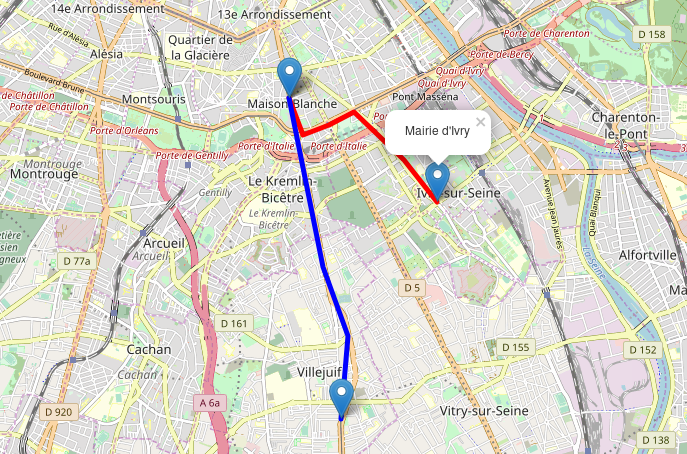
\includegraphics[width=\linewidth]{trajet.png}
  \caption{Trajet Villejuif-Louis Aragon \`a Mairie d'Ivry}
  \label{fig:trajet}
\end{figure}

\section{Les difficult\'es}
Durant ce projet, des difficult\'es se sont pr\'esent\'ees. L'algorithme pour
 trouver un trajet suppose que le voyageur a une petit patience pour \^etre
 rapide, le voyageur attend 4 heures au plus pour prendre un v\'ehicule.
 Malheuresement l'algorithme cherche un voyage sans transfert qui lie deux
 points d'arr\^et comme Mairie d'Ivry et Villjuif-Louis Aragon, mais un tel
 voyage n'existe pas. Donc l'algorithme v\'erifie tous les voyages ce qui le
 rend pas pratique.

\section{Conclusion}
Pour conclure, l'implementation actuelle arrive \`a trouver un trajet optimal
 rapidement si le voyageur est peu patience sinon le temps de calcul est
 deraisonable. Une id\'ee pour r\'esoudre ce probl\`eme est d'utiliser une
 liste chain\'ee.

\begin{thebibliography}{9}
\bibitem{GTFS}Reference de GTFS
  \url{https://developers.google.com/transit/gtfs/reference/}

\bibitem{RATP}La RATP vient de se lancer
  \url{http://www.lilletransport.com/Ouvrir-les-donnees-transport-de,149.html?lang=fr}

\bibitem{folium}Python Data, Leaflet.js Maps
  \url{https://pypi.org/project/folium/}

\bibitem{RATP_GTFS}Offre transport de la RATP - format GTFS
  \url{https://data.ratp.fr/explore/dataset/offre-transport-de-la-ratp-format-gtfs/information/}

\bibitem{Dijkstra}Dijkstra algorithm: How to implement it with Python (solved with all explanations) ?
  \url{http://www.gilles-bertrand.com/2014/03/dijkstra-algorithm-python-example-source-code-shortest-path.html}
\end{thebibliography}

\end{document}
